
\definecolor{c26497f}{RGB}{38,73,127}
\definecolor{cb20000}{RGB}{178,0,0}
\definecolor{ca3b3cc}{RGB}{163,179,204}


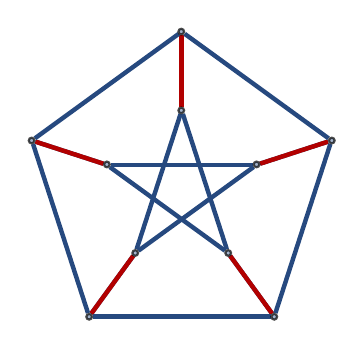
\begin{tikzpicture}[y=0.80pt,x=0.80pt,yscale=-1, inner sep=0pt, outer sep=0pt, scale=0.4]
\begin{scope}[shift={(0,0)}]
  \begin{scope}[cm={{1.0,0.0,0.0,1.0,(0.0,0.0)}}]
    \path[draw=c26497f,line width=1.600pt] (260.6910,162.8940) --
      (130.6130,257.4020);
    \path[draw=c26497f,line width=1.600pt] (259.8930,160.4380) --
      (99.1074,160.4380);
    \path[draw=c26497f,line width=1.600pt] (268.0450,159.1470) -- (344.6680,134.2510);
    \path<2->[draw=cb20000,line width=1.600pt] (268.0450,159.1470) -- (344.6680,134.2510);
    \path[draw=c26497f,line width=1.600pt] (228.3870,257.4020) --
      (98.3094,162.8940);
    \path[draw=c26497f,line width=1.600pt] (230.4770,255.8840) --
      (180.7910,102.9680);
    \path[draw=c26497f,line width=1.600pt] (234.2240,263.2380) -- (281.5790,328.4170);
    \path<2->[draw=cb20000,line width=1.600pt] (234.2240,263.2380) -- (281.5790,328.4170);
    \path[draw=c26497f,line width=1.600pt] (128.5230,255.8840) --
      (178.2090,102.9680);
    \path[draw=c26497f,line width=1.600pt] (124.7760,263.2380) --
      (77.4206,328.4170);
    \path<2->[draw=cb20000,line width=1.600pt] (124.7760,263.2380) --
      (77.4206,328.4170);
    \path[draw=c26497f,line width=1.600pt] (90.9554,159.1470) -- (14.3321,134.2510);
    \path<2->[draw=cb20000,line width=1.600pt] (90.9554,159.1470) -- (14.3321,134.2510);
    \path[draw=c26497f,line width=1.600pt] (179.5000,94.8159) -- (179.5000,14.2494);
    \path<2->[draw=cb20000,line width=1.600pt] (179.5000,94.8159) -- (179.5000,14.2494);
    \path[draw=c26497f,line width=1.600pt] (347.3510,136.9340) --
      (285.3260,327.8240);
    \path[draw=c26497f,line width=1.600pt] (345.2610,130.5040) --
      (182.8800,12.5270);
    \path[draw=c26497f,line width=1.600pt] (279.8570,331.7980) --
      (79.1429,331.7980);
    \path[draw=c26497f,line width=1.600pt] (73.6735,327.8240) -- (11.6494,136.9340);
    \path[draw=c26497f,line width=1.600pt] (13.7386,130.5040) -- (176.1200,12.5270);
    \path[fill=ca3b3cc] (264.0000,160.0000) ellipse (0.0897cm and 0.0897cm);
    \path[draw=black,draw opacity=0.700,line width=0.800pt] (264.0000,160.0000)
      ellipse (0.0897cm and 0.0897cm);
    \path[fill=ca3b3cc] (232.0000,260.0000) ellipse (0.0897cm and 0.0897cm);
    \path[draw=black,draw opacity=0.700,line width=0.800pt] (232.0000,260.0000)
      ellipse (0.0897cm and 0.0897cm);
    \path[fill=ca3b3cc] (127.0000,260.0000) ellipse (0.0897cm and 0.0897cm);
    \path[draw=black,draw opacity=0.700,line width=0.800pt] (127.0000,260.0000)
      ellipse (0.0897cm and 0.0897cm);
    \path[fill=ca3b3cc] (95.0000,160.0000) ellipse (0.0897cm and 0.0897cm);
    \path[draw=black,draw opacity=0.700,line width=0.800pt] (95.0000,160.0000)
      ellipse (0.0897cm and 0.0897cm);
    \path[fill=ca3b3cc] (179.0000,99.0000) ellipse (0.0897cm and 0.0897cm);
    \path[draw=black,draw opacity=0.700,line width=0.800pt] (179.0000,99.0000)
      ellipse (0.0897cm and 0.0897cm);
    \path[fill=ca3b3cc] (349.0000,133.0000) ellipse (0.0897cm and 0.0897cm);
    \path[draw=black,draw opacity=0.700,line width=0.800pt] (349.0000,133.0000)
      ellipse (0.0897cm and 0.0897cm);
    \path[fill=ca3b3cc] (284.0000,332.0000) ellipse (0.0897cm and 0.0897cm);
    \path[draw=black,draw opacity=0.700,line width=0.800pt] (284.0000,332.0000)
      ellipse (0.0897cm and 0.0897cm);
    \path[fill=ca3b3cc] (75.0000,332.0000) ellipse (0.0897cm and 0.0897cm);
    \path[draw=black,draw opacity=0.700,line width=0.800pt] (75.0000,332.0000)
      ellipse (0.0897cm and 0.0897cm);
    \path[fill=ca3b3cc] (10.0000,133.0000) ellipse (0.0897cm and 0.0897cm);
    \path[draw=black,draw opacity=0.700,line width=0.800pt] (10.0000,133.0000)
      ellipse (0.0897cm and 0.0897cm);
    \path[fill=ca3b3cc] (179.0000,10.0000) ellipse (0.0897cm and 0.0897cm);
    \path[draw=black,draw opacity=0.700,line width=0.800pt] (179.0000,10.0000)
      ellipse (0.0897cm and 0.0897cm);
  \end{scope}
\end{scope}

\end{tikzpicture}
